\chapter{Hardware Trojans}
First of all, lets give a definition of what a hardware trojan is.
\begin{boxH}
  A \textbf{hardware Trojan} (HT) is a malicious, intentional modification of a circuit design that
  results in undesired behavior when the circuit is deployed
\end{boxH}
SoCs that are ‘infected’ by a hardware Trojan may: 
\begin{itemize}
  \item experience changes in their functionality or specification 
  \item leak sensitive information,
  \item experience degraded or unreliable performance.
\end{itemize}
Hardware Trojan poses a serious threat to any hardware design being deployed in a critical
operation, in fact the most targeted systems are those that are used in military, generic critical
infrastructure(power plants, nuclear power plants,\dots) and financial systems.\\

Often, hw trojans includes \textbf{two main parts}: a \textbf{trigger} and a \textbf{payload}. The
A Trojan \textit{trigger} is an \textbf{optional part} that monitors various signals and/or a series
of events in the circuit. The payload usually taps signals from the original (Trojan-free) circuit
and the output of the trigger. Once the trigger detects an expected event or condition, the payload
is activated to perform malicious behavior.\\
Typically, the trigger is expected to be activated under extremely rare conditions, so the payload
remains inactive most of the time. This makes them extremely difficult to detect, mostly because ICs
have a complex design.

\begin{figure}[H]
  \centering
  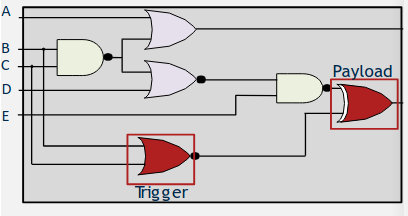
\includegraphics[width=0.6\textwidth]{img/hardware/hw trojan gates.png}
  \caption{Hardware Trojan at gate level}
  \label{fig:hw-trojan-gates}
\end{figure}

\begin{section}{Design Flow Process \& Vulnerabilities}
  We can distinguish three phases of the Design Flow Process:
  \begin{enumerate}
    \item \textbf{Pre-silicon}: it involves the design, testing, and tools. Vulnerabilities can come
      from:
      \begin{itemize}
        \item Untrusted 3rd party IPs.
        \item Untrusted CAD tools.
        \item Untrusted automation scripts.
        \item Untrusted libraries.
      \end{itemize}
    \item \textbf{Silicon}: in this phase, untrusted foundries can insert HT, such as:
      \begin{itemize}
        \item Ring Oscillator trojans.
        \item Backdoor circuits.
      \end{itemize}
    \item \textbf{Post-silicon}: at the final phase malicious packaging elements can be used to
      disguise a HT as a legitimate component.
  \end{enumerate}
  In any case, extra circuitry must be added to the design, which can lead to:
  \begin{itemize}
    \item Malfunctions.
    \item Leakage of secret information.
    \item Creation of backdoors for future attacks.
  \end{itemize}
  \begin{subsection}{IC Design Flow}
    The IC Design Flow is composed of five stages:
    \begin{enumerate}
      \item \textbf{Source-level RTL}: the RTL (Register Transfer Level) is usually defined
        in-house, while the IPO (Input, Process \& Output) is a 3rd party Soft IPO.
      \item \textbf{"Firm" RTL}: at this stage the Verilog netlist is synthesized and is now
        difficult to modify.
      \item \textbf{Gate-level Netlist}: defined using a Synthesis Tool.
      \item  \textbf{Physical Design}: the Place \& Route process is performed using a P\&R Tool. Some
        3rd party Hard IPs may be included at the end of it.
      \item \textbf{Packaging}: it is the final stage at the end of which, the finished chip is
        available.
    \end{enumerate}
    \begin{figure}[H]
      \centering
      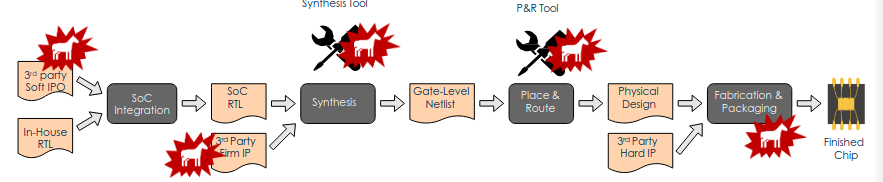
\includegraphics[width=0.8\textwidth]{img/hardware/ic design flow trojan.png}
      \caption{IC Design Flow}
      \label{fig:hw-trojan-design-flow}
    \end{figure}
     HTs could be inserted at any stage, especially those involving:
     \begin{itemize}
       \item Soft/Firm RTL.
       \item Hard IPs.
       \item CAD Tools.
       \item Packaging/Chiplets.
     \end{itemize}

     \begin{subsubsection}{Soft IP Trojans}
       Soft IP Trojans are written \textbf{directly in RTL}, either by an insider or a 3rd party.
       Their functionalities are undocumented, thus: They are hard to detect (especially in large
       projects) even with testing and/or simulation, furthermore, code reviews are tedious and
       expensive.
     \end{subsubsection}
     \begin{subsubsection}{Firm 3rd Party IP Trojans}
       Firm 3rd Party IP Trojans are \textbf{inserted} into the \textbf{Synthesized Netlist}, either
       manually or from the Source-level RTL. They can also be obfuscated, which makes them hard to
       Reverse Engineer.
     \end{subsubsection}
     \begin{subsubsection}{Malicious CAD Tool Trojans}
       CAD Tools are complex, and this makes it difficult to reason about logic optimizations.
       An attacker could then insert an additional logic and still remain undetected.\\
       Note: to achieve this, the HT’s Payload and Trigger must be limited in order to let the CAD
       understand the design well enough to known where to place the HT.
     \end{subsubsection}
     \begin{subsubsection}{Hard IP \& Foundry Trojans}
       IP Blocks are usually received as a VLSI Black Box, but makes the Physical Design of the IP
       hidden. However, Foundries may still edit the circuit’s design by:
       \begin{itemize}
         \item Adding wires to masks.
         \item Inserting additional standard cells.
       \end{itemize}
       Note: this is a difficult, but not impossible, process that typically requires Reverse
       Engineering of the Physical Design.
     \end{subsubsection}
  \end{subsection}
\end{section}

\begin{section}{Hardware Trojan Classifications}
  Hardware trojans can be classified as in figure \ref{fig:hw-trojan-classification}.
  \begin{figure}[H]
    \centering
    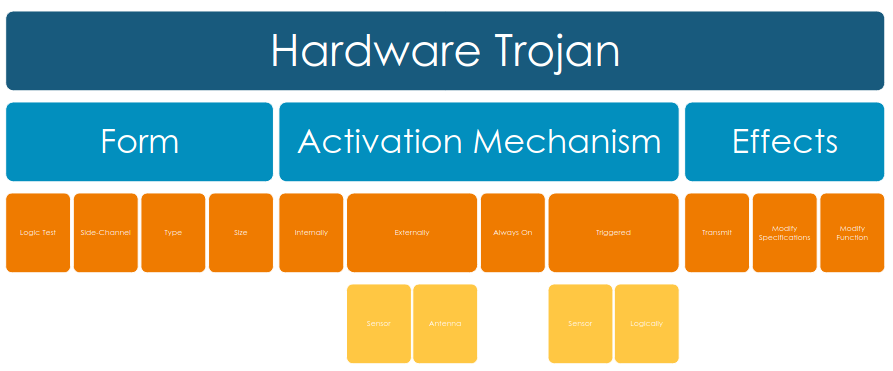
\includegraphics[width=\textwidth]{img/hardware/hw trojan classification.png}
    \caption{Hardware Trojan Classification}
    \label{fig:hw-trojan-classification}
  \end{figure}
\end{section}

\begin{section}{Hardware Trojan Detection}
Detecting a hardware trojan requires overcoming numerous challenges:
\begin{itemize}
  \item Handling many designs
  \item Being non-destructive to the IC
  \item Being cost-effective
  \item Ability to Detect trojans of different sizes or complexities
  \item Authenticating chips in as small a time frame as possible
  \item Robust variations in manufacturing processes
  \item Among others
\end{itemize}
Nowadays, there is a \textbf{lack of general HT detection techniques} or frameworks and most of the
ones who already exist cannot guarantee HT detection. Moreover, test time is expensive and HT are
designed to be stealthy.

\begin{figure}[H]
  \centering
  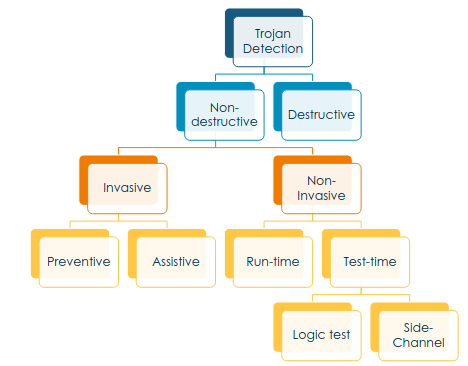
\includegraphics[width=0.5\textwidth]{img/hardware/hw trojan detection.png}
  \caption{Hardware Trojan Detection}
  \label{fig:hw-trojan-detection}
\end{figure}

\begin{subsection}{Direct I/O Access}
    Direct I/O is an obeying protocol that is used to send extra data in the circuit. Their I/O
    functionalities are undocumented, but typically include:
    \begin{itemize}
      \item Negative clock edges.
      \item Transmission happens only during "settling" periods.
    \end{itemize}
\end{subsection}

\begin{subsection}{EM Side Channel Information Leakage}
  Side Channels can be used to measure the IC’s EM radiation. Each wire of the IC acts as a
  mini-antenna and, since there are a lot of wires in the IC, the IC itself could be designed to
  (also) radiate a specific EM pattern/frequency.
\end{subsection}

\end{section}

\begin{section}{Hardware Trojan Mitigations}
  As you can see from figure \ref{fig:hw-trojan-mitigation}, there two main ways to mitigate HTs:
  pre and post silicon.
  \begin{figure}[H]
    \centering
    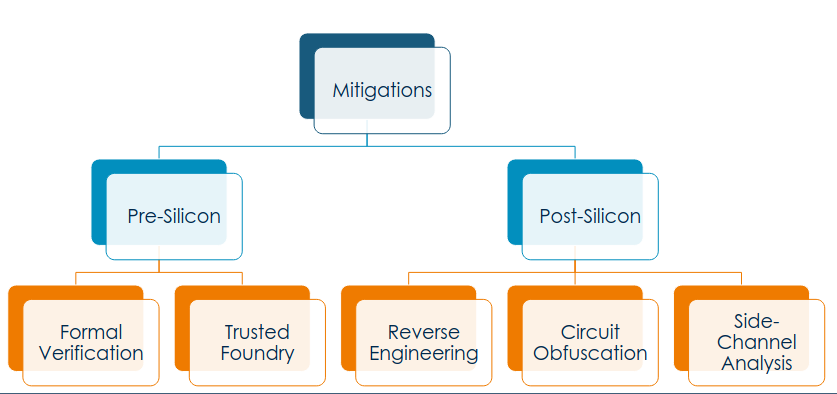
\includegraphics[width=0.8\textwidth]{img/hardware/hw trojan mitigation.png}
    \caption{Hardware Trojan Mitigation}
    \label{fig:hw-trojan-mitigation}
  \end{figure}
  \begin{subsection}{Reverse Engineering}
    Reverse Engineering is a HT mitigation techniques which can be always performed in the
    Post-silicon Design Flow phase. It consists in visually checking that the manufactured design
    matches the provided schematic.
    Visual checks require X-ray Inspection machines with whom we can inspect:
    \begin{itemize}
      \item PCB traces.
      \item IC bond wires.
    \end{itemize}
  \end{subsection}

  \begin{subsection}{Circuit Obfuscation}
    Circuit Obfuscation is a HT mitigation techniques which can be always performed in the
    Post-silicon Design Flow phase. It consists in hiding the true purpose of the circuit from the
    manufacturer. Circuit Obfuscation can be performed in two main ways:
    \begin{itemize}
      \item FPGA-based Implementation: the Foundry never gets the design.
      \item XOR Obfuscation: the Foundry gets the design, but not the XORing key. This technique can
        Obfuscate the whole circuit, or just a part of it.
    \end{itemize}
  \end{subsection}

  \begin{subsection}{Split Manufacturing}
    Split Manufacturing consists in fabricating the chip in multiple layers, so that no single
    Foundry has the whole design.

  \end{subsection}

\end{section}
